\documentclass{article}

\usepackage{arxiv}

\usepackage[utf8]{inputenc} % allow utf-8 input
\usepackage[T1]{fontenc}    % use 8-bit T1 fonts
\usepackage{hyperref}       % hyperlinks
\usepackage{url}            % simple URL typesetting
\usepackage{booktabs}       % professional-quality tables
\usepackage{amsmath}        % \text in math mode, align, etc.
\usepackage{amsfonts}       % blackboard math symbols
\usepackage{nicefrac}       % compact symbols for 1/2, etc.
\usepackage{microtype}      % microtypography
\usepackage{graphicx}
\usepackage{subcaption}     % subfigures
\usepackage{xcolor}         % colored TODO placeholders
\usepackage{array}
\usepackage[numbers,super,sort&compress]{natbib} % numbered superscript citations
\usepackage{doi}

% Visible placeholder for text, numbers or figures not yet available.
\newcommand{\TODO}[1]{\textcolor{red}{[\textbf{TODO:} #1]}}
% Hexadecimal addresses and tile ids.
\newcommand{\hex}[1]{\texttt{\$#1}}

\graphicspath{{figures/}{./}}

% Working title. Alternatives to discuss:
%  - "Same game, fewer pixels: a semantically simplified Super Mario Bros. for human and machine vision"
%  - "Controlling visual complexity in naturalistic video-game fMRI without changing the game"
\title{A visually simplified \textit{Super Mario Bros.} with identical game logic: a controlled stimulus for human and artificial gameplay}

\date{\today}

\author{ \href{https://orcid.org/0000-0002-8970-1983}{
\includegraphics[scale=0.06]{orcid.pdf}\hspace{1mm}Yann Harel}~$^{1,2,\ast}$ \\
	\And
	\href{https://orcid.org/0000-0002-4391-3075}{
\includegraphics[scale=0.06]{orcid.pdf}\hspace{1mm}Basile Pinsard}~$^{1,2}$ \\
    \And
	\href{https://orcid.org/0000-0001-5927-221X}{
\includegraphics[scale=0.06]{orcid.pdf}\hspace{1mm}Julie A. Boyle}~$^{1,2}$ \\
    \And
	\href{https://orcid.org/0000-0002-9111-0699}{
\includegraphics[scale=0.06]{orcid.pdf}\hspace{1mm}Lune Bellec}~$^{1,2}$ \\
}
% TODO: confirm author list and order (e.g. contributors to the RAM map and to the RL benchmarks).

\renewcommand{\shorttitle}{Simplified Super Mario Bros. stimulus}
\renewcommand{\headeright}{Preprint}
\renewcommand{\undertitle}{Preprint}

\hypersetup{
pdftitle={A visually simplified Super Mario Bros. with identical game logic},
pdfsubject={q-bio.NC, cs.CV},
pdfauthor={Yann Harel},
pdfkeywords={visual complexity, naturalistic stimuli, video games, fMRI, reinforcement learning, NES},
}

\begin{document}
\maketitle

\noindent
$^{1}$Centre de Recherche de l'Institut Universitaire de Gériatrie de Montréal, Montréal, QC, Canada.\\
$^{2}$Université de Montréal, Montréal, QC, Canada.\\
$^{\ast}$Corresponding author: Yann Harel (\texttt{yharel109@gmail.com}).

\begin{abstract}
Video games are increasingly used as naturalistic stimuli in neuroscience and as benchmarks
in artificial intelligence, but their rich visuals confound the study of task-relevant
processing: a player's behaviour and a brain's response depend jointly on what the game
\emph{requires} and on how it \emph{looks}. We present a modified version of the NES game
\textit{Super Mario Bros.} in which the visual scene is reduced to its functional content while
the game itself is left untouched. Every decorative element (clouds, hills, bushes, trees,
fences, castle, water plants) is made transparent, and every object the player can interact
with (ground, bricks, question blocks, coins, pipes, platforms, enemies, items, the player, the
goal) is drawn as a flat square whose colour encodes its semantic category identically in every
level. The modification rewrites only the graphics memory and the palette tables of the game
cartridge; program code, level data and random-number generation are unchanged. We verify on
participant recordings from the Courtois NeuroMod \textit{mario} dataset that the simplified
game replays controller inputs frame-for-frame identically to the original, that savestates are
interchangeable between the two versions, and that all RAM-derived behavioural variables are
preserved. The simplified game therefore provides a within-subject visual-complexity control
for existing and future gameplay recordings, for fMRI, and for reinforcement-learning agents.
\TODO{add one sentence on quantitative image-statistics results (edge density, spectral slope,
number of distinct colours) once computed.} \TODO{add one sentence on the planned fMRI / RL
experiment and its outcome.} The ROM generator, verification tools and the stimulus are released
openly.
\end{abstract}

\keywords{visual complexity \and naturalistic stimuli \and video games \and Super Mario Bros. \and fMRI \and reinforcement learning}


\section{Introduction}
\label{sec:intro}

\TODO{Paragraph 1 -- naturalistic paradigms and video games as stimuli: continuous audiovisual
input, goal-directed motor action, measurable performance and learning; CNeuroMod
\textit{mario}\cite{paugam2025mario} and \textit{shinobi}\cite{harel2025shinobi} datasets; games
as RL benchmarks (Gym Retro\cite{openai2018gymretro}).}

\TODO{Paragraph 2 -- the confound: visual richness vs. task structure. In a naturalistic game,
low-level visual features (edges, textures, colour variety, motion of background parallax),
mid-level object appearance (shape, animation) and task-relevant semantics (what is solid, what
is dangerous, what is collectible) covary. Brain responses and agent policies can be driven by any
of them. Existing approaches either change the task (abstract games such as VGDL / Procgen) or
change the stimulus without controlling the task (movies vs. line drawings). Cite visual
complexity / clutter measures and object-vs-feature literature.}

\TODO{Paragraph 3 -- what we did: a version of \textit{Super Mario Bros.} whose visual scene is
stripped of decoration and whose interactive objects are rendered as colour-coded squares, with
provably identical game logic. Mention that the \textit{mariostars} dataset already provides the
opposite manipulation (richer 16-bit graphics, same levels)\cite{paugam2025mario}, so that
together the three versions span a visual-complexity axis around the same task.}

\TODO{Paragraph 4 -- contributions: (i) the method, applicable to any NES title with a mapper-0
cartridge and to other 8/16-bit systems with tile-based graphics; (ii) the verification protocol
(replay and savestate identity); (iii) the released stimulus, generator and tools; (iv)
quantitative characterisation of the visual change; (v) planned experiments.}


\section{Methods}
\label{sec:methods}

\subsection{Design goals}
\label{sec:goals}

The simplified game was designed under three constraints.
\begin{enumerate}
  \item \textbf{Functional transparency.} Any element with no effect on gameplay is removed from
  the image, i.e.\ rendered as the uniform backdrop. This includes clouds, hills, bushes,
  background trees and trunks, fences, chains, bridge guard-rails, the water surface line,
  sea plants, balance-lift ropes and pulleys, the end-of-level castle, fireworks and brick
  debris.
  \item \textbf{Semantic colour coding.} Every element the player can interact with is drawn as
  a flat square of a single colour, and the colour is a semantic category that is the same in
  every level regardless of the original day, night, underground or water palette
  (Table~\ref{tab:legend}).
  \item \textbf{Logical identity.} Program code, physics, level layouts, enemy behaviour, RAM
  layout and random-number generation are untouched, so that controller recordings and savestates
  made on the original game remain valid on the simplified one, RAM-derived behavioural variables
  are identical, and humans and agents face exactly the same task.
\end{enumerate}

\begin{table}[t]
  \caption{Semantic colour legend of the simplified game. NES master-palette indices are given in
  hexadecimal. Colours are configurable in the generator.}
  \centering
  \small
  \begin{tabular}{llp{9.2cm}}
    \toprule
    Category & Colour (NES) & Objects \\
    \midrule
    background & sky blue (\hex{22}) & everything non-interactive, in every area type \\
    terrain & brown (\hex{17}) & ground, stairs, hard blocks, pipes, tree-top and mushroom ledges, cloud terrain, cannons, bridges, used blocks, moving platforms, springboards, bumped bricks \\
    brick & grey (\hex{10}) & breakable bricks \\
    ?-block & orange (\hex{27}) & question blocks, including the sprite of a bumped question block \\
    coin & yellow (\hex{28}) & coins in the level and coins popping out of blocks \\
    item & green (\hex{2A}) & mushroom, 1-up, fire flower, star, vine \\
    enemy & red (\hex{16}) & every enemy and enemy projectile (hammers, bullets) \\
    player & white (\hex{30}) & Mario; flashes white / green / orange under star power \\
    fire player & pale pink (\hex{36}) & Mario after a fire flower, and his fireballs \\
    goal & purple (\hex{24}) & flagpole, ball, flag, axe \\
    \bottomrule
  \end{tabular}
  \label{tab:legend}
\end{table}

\subsection{The original stimulus}
\label{sec:original}

The reference game is the NTSC release of \textit{Super Mario Bros.} (Nintendo, 1985) as
distributed in the CNeuroMod \textit{mario} stimulus set\cite{paugam2025mario}, run under the
\texttt{fceumm} core\cite{fceumm} of \texttt{stable-retro}\cite{stableretro}, a maintained fork
of Gym Retro\cite{openai2018gymretro}. The stimulus set defines 22 playable levels (worlds 1--8,
stages 1--3; castle and water levels were excluded from the dataset) through emulator savestates,
a reward/termination scenario, and a map of RAM addresses to named variables (player position,
score, coins, lives, enemy states, power-up state, level and area identifiers). Participants'
gameplay is stored as \texttt{.bk2} files: the emulator's initial state plus the controller input
of every frame at 60~Hz, which the deterministic emulator turns back into the full audiovisual
stream and RAM trajectory. \TODO{cite the dataset numbers: 5 participants, 22 levels, N
repetitions, hours.}

\subsection{How the NES draws the game, and why it can be recoloured without changing it}
\label{sec:nes}

An NES cartridge holds two read-only memories\cite{nesdev}. \emph{PRG-ROM} (32~KB for this
title) contains the 6502 program, the level data and a number of small data tables.
\emph{CHR-ROM} (8~KB) contains the pixel shapes of 512 tiles of $8\times8$ pixels at 2~bits per
pixel: 256 tiles for sprites (moving objects) and 256 for the background. Colour is not stored in
the tiles: each pixel value 0--3 is an index into one of eight 4-colour palettes (four for the
background, four for sprites) held by the picture processing unit (PPU); index 0 is transparent
for sprites and the shared backdrop colour for the background.

The game never reads CHR-ROM: it only tells the PPU which tile to draw where. Collision,
movement, scoring and every other rule operate on \emph{metatile} identifiers (16$\times$16-pixel
block types) and object identifiers held in RAM, not on pixels. Palettes are only \emph{written}
by the game, at level load and for a few animations, from small tables in PRG-ROM, through a
write buffer in RAM (\hex{0300}--\hex{03FF}) that is flushed to the PPU during vertical blank.
Nothing in the game reads the palette back. Two consequences follow. Rewriting CHR-ROM changes
what is seen and nothing else. Rewriting the palette tables in PRG-ROM (and, as detailed below,
one table mapping metatiles to tiles and four constants selecting an object's sprite palette)
changes only the bytes that pass through the PPU write buffer and the sprite list, with no effect
on game state. Section~\ref{sec:verification} tests this claim empirically rather than relying on
it.

\subsection{Background tiles}
\label{sec:bg}

\textit{Super Mario Bros.} composes the background from metatiles, each defined by four tile
identifiers listed in four tables in PRG-ROM (one table per background palette, 101 metatiles in
total; CPU addresses \hex{8B10}--\hex{8CC0} in the annotated disassembly\cite{smbdis}). We dumped
these tables from the original ROM and used them to assign every background tile to the block
type(s) it belongs to (ground, brick, question block, pipe, cloud, bush, hill, \ldots), rather
than guessing from its picture. Each tile was then rewritten as either transparent (all pixels
index~0) for decoration, or a solid square of a chosen palette index (1, 2 or 3) for interactive
blocks; the index selects the semantic colour through the palettes of Section~\ref{sec:palettes}.
The flagpole shaft keeps its thin shape but is recoloured, and text and HUD tiles are untouched.
Figure~\ref{fig:tilesheet} shows the complete tile sheet before and after.

Two tiles are shared between categories and could not be both transparent and solid. Tile
\hex{26} is both the fill of the decorative hills and the inner column of every pipe shaft; tile
\hex{47} is both the breakable brick and the wall of the end-of-level castle. We therefore also
edited the metatile-graphics table: the two pipe-shaft metatiles use the pipe-edge tile instead of
\hex{26} (4 bytes), and the seven castle metatiles use the blank tile (28 bytes), which makes the
castle, a purely decorative object, disappear. This table is read only when the game writes a new
screen column into the PPU write buffer.

\subsection{Sprite tiles}
\label{sec:sprites}

Every sprite tile below \hex{F6} becomes a solid square (the floating score digits
\hex{F6}--\hex{FF} are kept). The index a tile receives depends on which object draws it, and
this was \emph{measured} rather than assumed. The game builds its sprite list in RAM
(\hex{0200}--\hex{02FF}) and keeps, for the player, each of six enemy slots (one of which hosts
the power-up object), bumped blocks, bubbles, fireballs and miscellaneous objects, the offset of
their entries (\hex{06E4}--\hex{06FB}); enemy identifiers and active flags are at
\hex{0016}--\hex{001B} and \hex{000F}--\hex{0014}. Replaying 66 participant recordings (three
per level, all 22 levels) on the original ROM and reading these locations every third frame gave,
for each of the 512 sprite tiles, the object that drew it and the sprite palette it was drawn
with. The resulting map covers the player (86 tiles), 14 enemy types, the four power-ups,
fireballs, coins, hammers, the flag, vines, moving platforms, springboards, fireworks and the
castle flag; tiles never observed default to the enemy category.

Because a sprite's palette is chosen by the game per object, tiles of different categories can
share a palette (the mushroom and the Spiny both use sprite palette~2, for instance). Categories
are therefore separated by \emph{index} within a palette (enemies index~2, items index~1,
platforms index~3), and the palettes of Section~\ref{sec:palettes} give each index its colour.
The player's tiles use index~1 because the star-power effect rotates the player's palette
\emph{attribute} through the four sprite palettes: with index~1 he flashes white, green, green
and orange rather than enemy red.

Four palettes with three indices each give twelve sprite colours, but the game's own palette
assignments crowd some categories into the same palette (coins popping out of blocks, fireballs,
the mushroom and the Spiny all use sprite palette~2). Where that prevented a category from having
its own colour, we changed the palette the game assigns to the object; each change is a single
immediate operand in that object's drawing routine (Table~\ref{tab:changes}). The fireball now
uses the player's palette (index~3), coins popping out of blocks use palette~3 (index~3), the
bumped brick uses palette~2 (index~3, terrain colour, as no sprite palette has a slot left for the
brick grey), and the bumped question block always uses palette~3 (the original used palette~1
outside ground areas). Brick debris sprites are transparent.

\subsection{Palettes}
\label{sec:palettes}

The game keeps four 32-byte palette sets (water, ground, underground, castle), three 4-byte
variants for snow and mushroom areas, a 12-byte player palette table (Mario, Luigi, fire Mario),
an 8-byte backdrop-colour table, and two small tables used to animate question blocks and coins by
rewriting background palette~3 every 8 frames. All of these were overwritten so that every
palette index means the same category everywhere (Table~\ref{tab:palettes}). The backdrop is
sky blue in every area, including underground and night levels. The fire-player colour
(\hex{36}, a pale pink) was chosen close to the player's white so that the change of state is
visible while keeping the object in the ``player'' family; fireballs share it.

\begin{table}[t]
  \caption{Meaning of each palette index after the modification. BG: background palettes; SPR:
  sprite palettes. Index 0 is the backdrop (background) or transparent (sprites).}
  \centering
  \small
  \begin{tabular}{lcccccccc}
    \toprule
    index & BG0 & BG1 & BG2 & BG3 & SPR0 & SPR1 & SPR2 & SPR3 \\
    \midrule
    1 & item & brick & text (white) & ?-block & player & item & item & ?-block \\
    2 & terrain & terrain & terrain & terrain & item & enemy & enemy & enemy \\
    3 & goal & goal & goal & coin & fire player & goal & terrain & coin \\
    \bottomrule
  \end{tabular}
  \label{tab:palettes}
\end{table}

\subsection{Summary of the binary changes}
\label{sec:changes}

Table~\ref{tab:changes} summarises the bytes that differ between the original and the simplified
cartridge image. No byte of program code or level data is changed; the 194 modified PRG-ROM bytes
are all data that the game copies into the PPU write buffer or the sprite list.

\begin{table}[t]
  \caption{Bytes changed in the cartridge image (40{,}976 bytes: 16-byte iNES header, 32~KB
  PRG-ROM, 8~KB CHR-ROM).}
  \centering
  \small
  \begin{tabular}{lrp{8.6cm}}
    \toprule
    Region & Bytes & Nature of the change \\
    \midrule
    iNES header & 0 & -- \\
    PRG-ROM: code and level data & 0 & -- \\
    PRG-ROM: palette tables & 158 & four area palette sets, snow and mushroom variants, Bowser palette, player palette rows, backdrop table, question-block/coin animation tables \\
    PRG-ROM: metatile graphics table & 32 & pipe shafts (4) and castle (28) \\
    PRG-ROM: sprite-palette operands & 4 & fireball, block coin, bumped brick, bumped ?-block \\
    CHR-ROM: tile shapes & 5{,}545 & 244 sprite tiles and 96 background tiles rewritten \\
    \bottomrule
  \end{tabular}
  \label{tab:changes}
\end{table}

\subsection{Reproducibility}
\label{sec:repro}

The simplified cartridge is generated deterministically from the original by a single script
(\texttt{code/simplify\_rom.py}) that contains the tile classification, the colour table and the
list of PRG patches; every PRG patch asserts the original bytes before writing. The input is the
original ROM of the \textit{mario} stimulus set (MD5 \texttt{811b027e\ldots}); the output has MD5
\texttt{6d5c5d99\ldots}. Two companion tools reproduce the sprite survey
(\texttt{survey\_sprite\_tiles.py}) and the verification of Section~\ref{sec:verification}
(\texttt{verify\_replays.py}). The stimulus is distributed as a drop-in replacement of the
\textit{mario} stimulus set: same savestates, scenario and RAM-variable map, different
\texttt{rom.nes}.

\subsection{Verification of logical identity}
\label{sec:verification}

We tested the claim of Section~\ref{sec:nes} directly. For a participant recording, the
controller input is replayed on the original and on the simplified ROM with the same emulator,
starting from the recording's own initial savestate, and the complete emulator RAM is compared
after every frame. Differences are only tolerated in three regions that the graphics path writes
and game logic never reads: the sprite list (\hex{0200}--\hex{02FF}), the PPU write buffer
(\hex{0300}--\hex{03FF}) and one zero-page scratch byte (\hex{0004}) in which the block-drawing
routine hands its palette to a shared helper. A savestate is also taken halfway through the run on
the original ROM, loaded into the simplified ROM, and the remaining input is replayed to check
that the run continues identically. The same procedure applied to a graphics-only build (tile
changes without any PRG patch) must yield byte-identical RAM on every frame, which tests the
emulator side of the argument.

\TODO{decide on the final verification set: currently six recordings (levels 1-1 with fire
Mario, star power and a completed level; 1-2; 1-3; 3-1; 4-2; 8-2; 2{,}800--6{,}000 frames each)
plus all 24 level savestates with scripted input. Consider running the full dataset (all
$\sim$3{,}400 recordings) and reporting the count.}

\subsection{Characterisation of the visual change}
\label{sec:imagestats}

\TODO{Define and compute image statistics on matched frames of the two versions (same recording,
same frame): edge density, number of distinct colours per frame, spatial-frequency spectral slope,
feature-congestion clutter, mean luminance and contrast, optical-flow magnitude, and per-frame
entropy. Report distributions over all frames of the dataset and per level. Also report the
proportion of the screen covered by transparent (backdrop) pixels before and after.}

\TODO{Describe the semantic-mask derivation: since colour now identifies category, a per-pixel
semantic segmentation of every frame is obtained for free by colour lookup. Validate it against
RAM-derived object positions.}

\subsection{Planned experiments}
\label{sec:planned}

\TODO{fMRI: acquire the same 22 levels with the simplified game in the same CNeuroMod
participants (design mirrors \textit{mario}; number of sessions to decide). Analyses: (a)
annotation-based GLM maps for the same gameplay conditions as \textit{mario} and
\textit{mariostars}, compared across the three visual versions of the same task; (b)
encoding models of low-level visual features vs. semantic-category features, testing which part
of the visual-cortex response transfers across versions; (c) behavioural learning trajectories
and transfer between versions.}

\TODO{Reinforcement learning: train PPO\cite{schulman2017ppo} agents (as in the
\textit{mario} stimulus metadata) on original vs. simplified graphics; measure sample efficiency,
final performance and cross-version transfer of policies trained on one version and evaluated on
the other; compare agent and human behaviour under both versions.}


\section{Results}
\label{sec:results}

\subsection{The simplified game}

Figure~\ref{fig:compare} shows matched frames of the two versions, and
Figure~\ref{fig:levels} the first screen of every level after 7~s of scripted play. Decorative
elements are absent, terrain and blocks are flat, and objects of the same category share a colour
across day, night and underground levels. \TODO{add one or two sentences describing what a naive
observer sees, and the object-size cue that replaces shape (a Goomba and small Mario are both
$16\times16$; a Koopa is $16\times24$; big Mario $16\times32$).}

\begin{figure}[t]
  \centering
  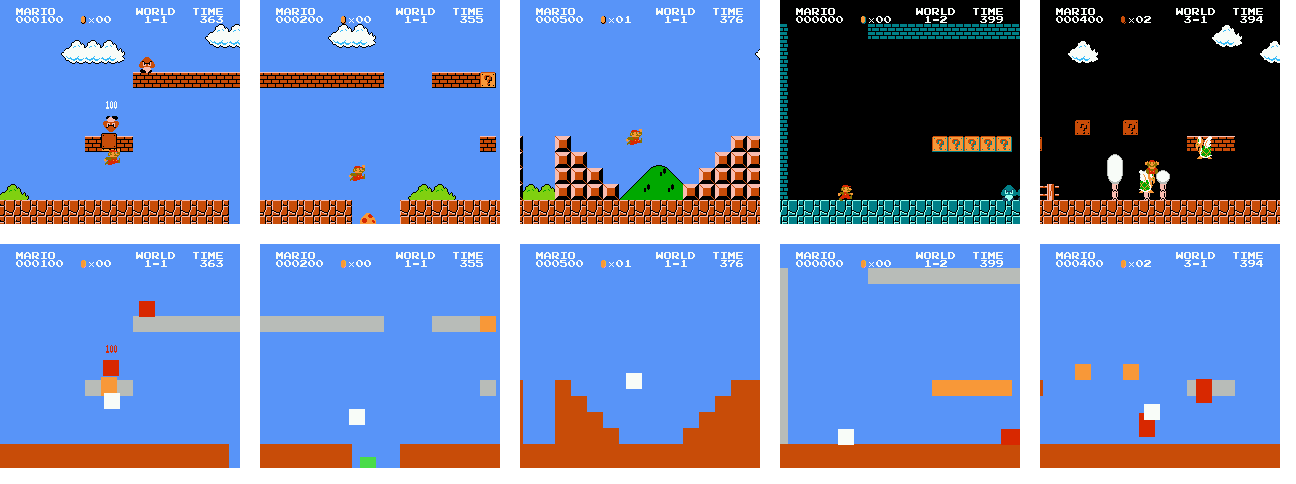
\includegraphics[width=\textwidth]{original_vs_simplified.png}
  \caption{Matched frames of the original (top) and simplified (bottom) game: three frames of a
  participant recording in level 1-1, and scripted play in the underground level 1-2 and the night
  level 3-1. \TODO{replace by a curated selection and add panel labels; consider adding the
  \textit{mariostars} rendering of the same frames as a third row.}}
  \label{fig:compare}
\end{figure}

\begin{figure}[t]
  \centering
  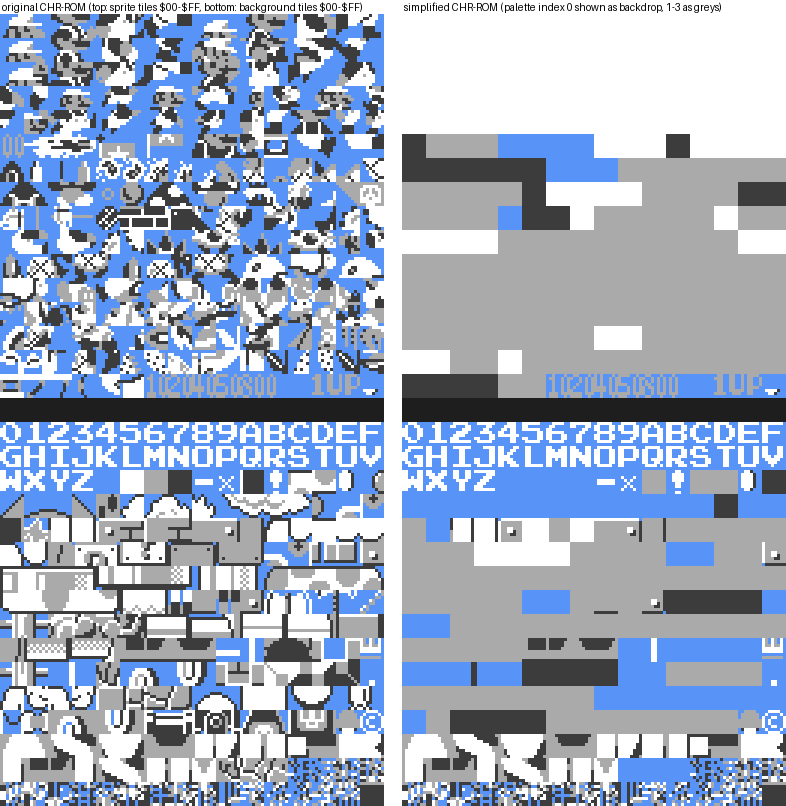
\includegraphics[width=0.8\textwidth]{tilesheet_original_vs_simplified.png}
  \caption{The complete CHR-ROM tile sheet before (left) and after (right) the modification.
  Top half: 256 sprite tiles; bottom half: 256 background tiles. Palette index 0 is shown in blue,
  indices 1--3 in greys. \TODO{annotate categories.}}
  \label{fig:tilesheet}
\end{figure}

\begin{figure}[t]
  \centering
  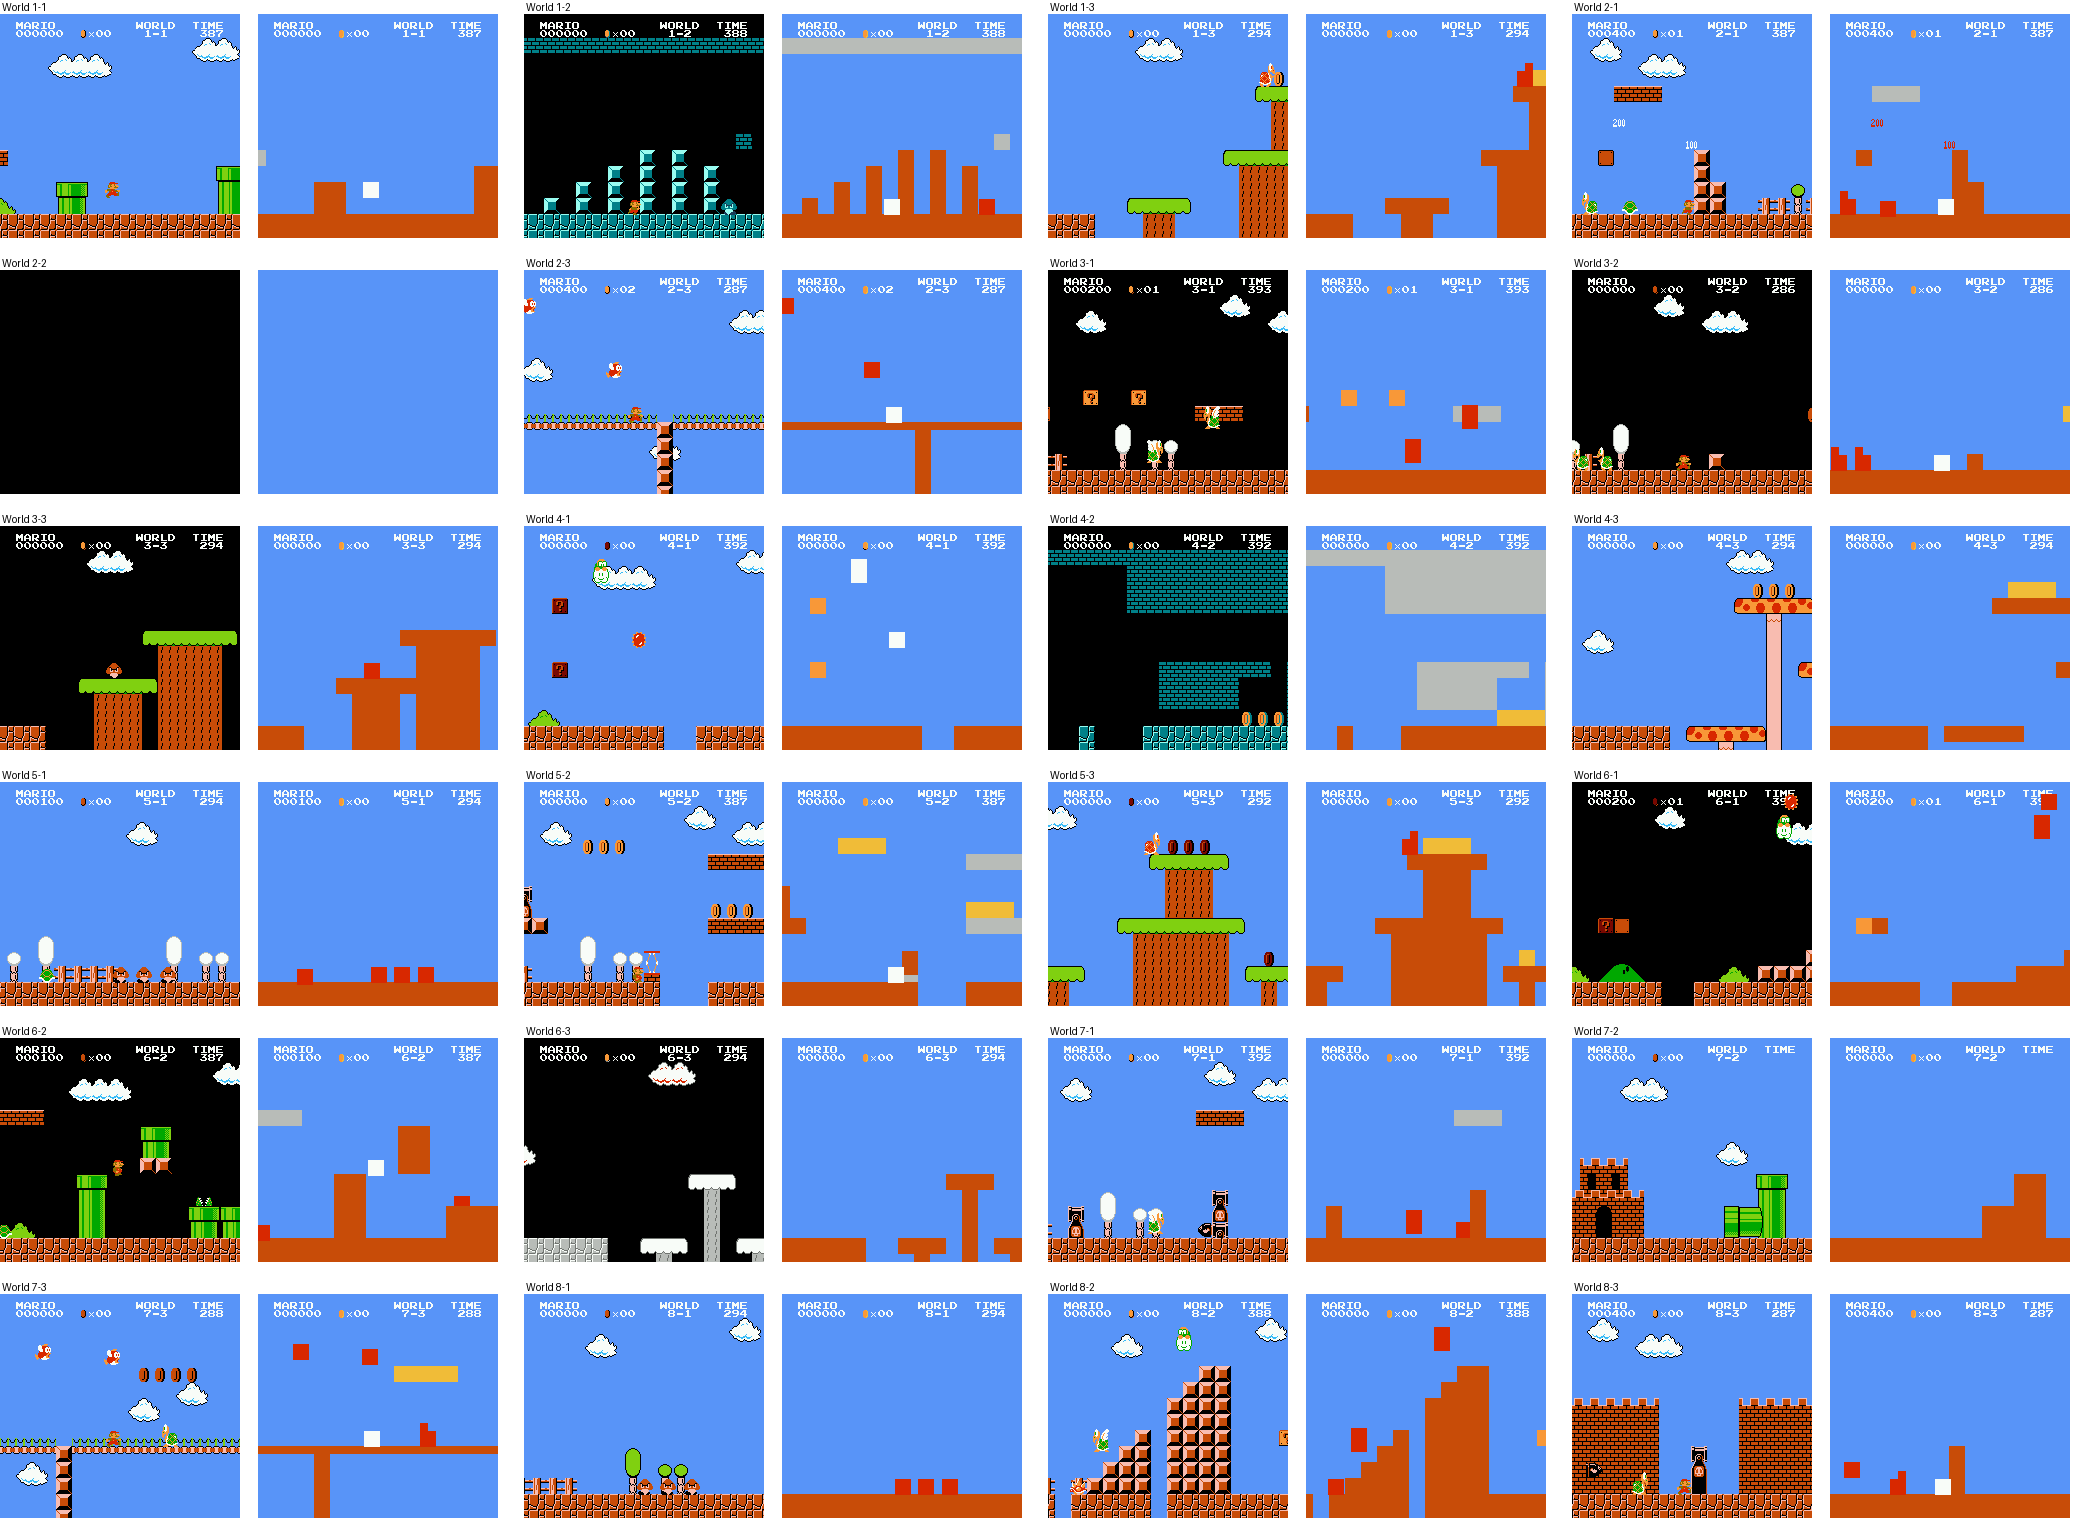
\includegraphics[width=\textwidth]{levels_original_vs_simplified.png}
  \caption{Original (left of each pair) and simplified (right) rendering of the 24 level savestates
  of the stimulus set after 420 frames of scripted input (run right, jump periodically).
  \TODO{move to supplementary material or select a subset.}}
  \label{fig:levels}
\end{figure}

\subsection{Logical identity}

\TODO{turn into a table.} On the six recordings tested, the graphics-only build produced
byte-identical RAM on every frame. With the palette, metatile and sprite-palette patches, the
only RAM bytes that ever differed lay in the three presentation regions listed in
Section~\ref{sec:verification} (\hex{0004}, \hex{0200}--\hex{02FF} and \hex{0304}--\hex{03B0}),
on the frames where a screen column, a palette or an affected sprite was queued; no byte outside
these regions differed on any frame, and savestates taken on either ROM loaded on the other and
tracked the original run to its end. Consequently every RAM-derived variable of the stimulus set
(positions, score, coins, lives, enemy and power-up states) is identical between versions for a
given input sequence, and the 3{,}374 recordings of the \textit{mario} dataset can be rendered in
either version without conversion. \TODO{confirm the recording count from the dataset paper.}

\subsection{Visual statistics}

\TODO{results of Section~\ref{sec:imagestats}, with a figure: distributions of edge density,
colour count and spectral slope for original / simplified / \textit{mariostars} frames.}


\section{Discussion}
\label{sec:discussion}

\TODO{What the stimulus enables: a three-level visual-complexity manipulation
(\textit{simple} / \textit{mario} / \textit{mariostars}) around a fixed task; within-subject
comparisons in the CNeuroMod cohort; a free semantic segmentation of every frame; a testbed for
the visual abstraction question in RL.}

\TODO{Design decisions and their rationale: colour as the only category cue; shape removed but
size retained; why the backdrop is uniform even underground; why bumped bricks are brown; why the
castle is removed; why star power still flashes.}

\TODO{Generality of the method: applies to any NES title (and, with the same logic, to other
tile-based consoles) provided the metatile/graphics tables can be located; the verification
protocol is game-agnostic. Limitations: shape information is lost entirely; objects that never
appear in the recorded levels default to the enemy colour; the HUD keeps the original font;
mid-level savestates keep the original palette until the next area load (a tool is provided to
rewrite them).}

\TODO{Relation to prior work on abstracted game stimuli and on visual clutter in perception.}


\section*{Code and data availability}
The simplified stimulus set, the generator, the sprite survey and the verification tools are
available at \url{https://github.com/courtois-neuromod/mario.simple} (\TODO{tag/commit at
release}). The original stimulus set is \url{https://github.com/courtois-neuromod/mario.stimuli}.
The participant recordings used for verification belong to the CNeuroMod \textit{mario}
dataset\cite{paugam2025mario}. \TODO{the ROM itself is copyrighted; describe how the stimulus is
distributed (git-annex restricted access, as for the original) and whether a patch file (IPS/BPS)
against the original ROM can be published instead.}

\section*{Acknowledgements}
\TODO{funding (Courtois foundation), participants, contributors to the RAM map.}

\section*{Author contributions}
\TODO{Y.H.\ conceived the stimulus, implemented the generator and verification, and wrote the
manuscript; B.P.\ built the original stimulus set and the deployment infrastructure; \ldots}

\section*{Competing interests}
The authors declare no competing interests.

\bibliographystyle{unsrtnat}
\bibliography{references}

\end{document}
